\documentclass[a4paper,openright, 10pt]{article}
\usepackage[utf8]{inputenc}
\usepackage{graphicx}
\usepackage{tikz}
\usetikzlibrary{datavisualization}
\usetikzlibrary{datavisualization.formats.functions}

\graphicspath{ {./images/} }

\usepackage{fullpage}
\newcommand{\ssection}[1]{%
\section[#1]{\centering\normalfont\scshape #1}}
\newcommand{\ssubsection}[1]{%
\subsection[#1]{\bfseries\normalfont\scshape #1}}
\newcommand{\ssubsubsection}[1]{%
\ssubsubsection[#1]{\bfseries\normalfont\scshape #1}}

\title{Study Guide}
\author{Team L.A.J., League of Anti Josh}
\date{Quarter 1}

\begin{document}

\maketitle
\section*{Table of Contents}\\
Integration by Parts...........................pg.1\\
Integration by Partial Fractions...............pg.4\\
Improper Integrals....................................pg.8\\
First Order Separable Differential Equations...pg.11\\
First Order Linear Differential Equations......pg.14\\
Slope Fields...................................pg.18\\
Euler's Method.................................pg.19\\
Logistic Model.................................pg.22\\
\ssection{Integration}
 \section*{Integration by Parts}
The formula for integration by parts can be found by manipulating the product rule. The result of this is a formula that can be used to find the anti-derivative of two functions being multiplied where u-substitution cannot be used. Let's look at how the formula can be derived.
\\\underline{Solving for Formula}
$$(u\cdot v)'=v\cdot u'+u\cdot v'$$
$$\int(u\cdot v)'=\int(v\cdot du+ u\cdot dv)$$
Integrate both sides of the equation to eliminate the derivative on the left side and make the function solvable for u times v.
$$uv=\int vdu + \int udv$$
$$uv-\int vdu=\int udv$$
Subtract the integral of $vdu$ from both sides to solve for the integral of $udv$ to get the integration by parts formula.\\
\underline{Formula}
$$\int udv= uv-\int vdu$$
\\
When using this formula, you'll want to be very careful in identifying what part of the integral you set equal to $u$ and $dv$. Sometimes you'll make the wrong choice and you'll have to go back and change what you set equal to $u$ and $dv$. Most times, you'll want to set the part of the integral that can eventually be derived equal to $u$. You'll set the other part of the integral equal to $dv$. To see how this works, let's try an example.\\
\\Examples:\\\\
\underline{Example 1}\\
$$\int lnxdx$$\\
First, we want to identify what to set equal to $u$ and what to set equal to $dv$. Since we know that we can find the derivative of $lnx$, we'll set this equal to $u$. Since it's easy to find the anti-derivative of $dx$, it makes sense to set it equal to $dv$.\\
$$(u=lnx\longrightarrow du=\frac{1}{x}dx)(dv=dx\longrightarrow v=x)$$
$$\int udv=uv-\int vdu$$
We'll substitute the values into the formula.\\
$$\int lnxdx=x\cdot lnx-\int x\cdot\frac{1}{x}dx$$
Simplify.\\
$$\int lnxdx=x\cdot lnx-\int dx$$
$$\fbox{\int lnxdx=x\cdot lnx-x+c}$$
\underline{Example 2}\\
$$\int x^2e^xdx$$
Since we know that the derivative of $x^2$ can eventually be found, we'll set that equal to $u$ and set $e^x$ equal to $dv$ because it's simple to find its anti-derivative.
$$(u=x^2\longrightarrow du=2xdx)(dv=e^xdx\longrightarrow v=e^x)$$
Substitute these values into the formula.\\
$$\int x^2e^xdx=x^2e^x-\int 2xe^xdx$$
We'll have to use integration by parts again to solve $\int 2xe^xdx$.\\
$$(u=2x\longrightarrow du=2dx)(dv=e^x\longrightarrow v=e^x)$$
$$\int x^2e^xdx=x^2e^x-(2xe^x-\int 2e^xdx)$$
$$\int x^2e^xdx=x^2e^x-(2xe^x-2e^x+c)$$
$$\fbox{\int x^2e^xdx=x^2e^x-2xe^x+2e^x+c}$$
This problem can also be quickly solved using a concept called the tabular method. It's made of a table with three columns. The first column shows $u$ and its derivatives. The second column shows $dv$ and its anti-derivatives. The third column flips between positive and negative, always starting with positive. To use the table, you multiply the values in each column in a downward diagonal motion, starting in the first column. For a better understanding, see the table below using the information from example 2.\\
\underline{Tabular Method}\\
\\
\begin{tabular}{c|c|c}
    u & dv & + or -\\
    \hline
    x^2 & e^x & +\\
    \hline
    2x & e^x & -\\
    \hline
    2 & e^x & +\\
    \hline
    0 & e^x & -\\
    \hline
     & &+\\
\end{tabular}\\
\\
If we multiply downwards diagonally, we can see that we end up getting $x^2e^x-2xe^x+2e^x$. Once we add $c$ to this, we can see that we get the same answer as we did in example 2. Using the tabular method is a much faster, simpler way to solve integrals with a value that can eventually be derived and a value that repeats in a cycle when derived such as $cosx$ or $e^x$.\\
\\
\underline{Example 3}
$$\int x^2sinxdx$$
This is another example that we can solve out by hand or with the tabular method. We'll try both ways, just to confirm that the tabular method works on problems involving trigonometry.\\
$$(u=x^2\longrightarrow du=2xdx)(dv=sinxdx\longrightarrow v=-cosx)$$
$$\int x^2sinxdx=-x^2cosx-\int -2xcosxdx$$
We have to use the integration by parts formula again.
$$(u=2x\longrightarrow du=2dx)(dv=-cosxdx\longrightarrow v=-sinx)$$
$$\int x^2sinxdx=-x^2cosx-(-2xsinx-\int -2sinxdx)$$
$$\int x^2sinxdx=-x^2cosx-(-2xsinx-2cosx+c)$$
$$\fbox{\int x^2sinxdx=-x^2cosx+2xsinx+2cosx+c}$$
\underline{Tabular Method}\\
\\
\begin{tabular}{c|c|c}
    u & dv & + or -\\
    \hline
    x^2 & sinx & +\\
    \hline
    2x & -cosx & -\\
    \hline
    2 & -sinx & +\\
    \hline
    0 & cosx & -\\
    \hline
     & &+\\
\end{tabular}\\
\\
By multiplying downwards diagonally, we get $-x^2cosx+2xsinx+2cosx$. If we add $c$ to this, we do get the same answer as we did in example 3.\\
\\
\underline{Example 4}
$$\int e^xcosxdx$$
$$(u=e^x\longrightarrow du=e^xdx)(dv=cosxdx\longrightarrow v=sinx)$$\\
For this problem, both values cycle and never reach a constant, so we have to experiment with setting $e^x$ equal to $u$ to try to allow the integral to reach a point in the cycle where it can be solved.
$$\int e^xcosxdx= e^xsinx-\int e^xsinxdx$$
We'll have to try integration by parts again.
$$(u=e^x\longrightarrow du=e^xdx)(dv=sinxdx\longrightarrow v=-cosx)$$
$$\int e^xcosxdx= e^xsinx-(-e^xcosx-\int -e^xcosxdx)$$
$$\int e^xcosxdx= e^xsinx+e^xcosx-\int e^xcosxdx$$
We can now add $\int e^xcosxdx$ to both sides to isolate $\int e^xcosxdx$.\\
$$2\int e^xcosxdx= e^xsinx+e^xcosx$$
Divide both sides by 2 to reach a final answer.\\
$$\fbox{\int e^xcosxdx= \frac{e^xsinx+e^xcosx}{2}}$$
 \section*{Integration by Partial Fractions}
 Intro:
 \\So, in integrating we come across certain integrals that we cannot find using traditional way, u-substitution, or integration by parts. The integrals that fit under this category and have huge fractions with polynomials in the denominator can be solved using impartial fractions.\\
 \\Examples:\\\\
 \underline{Example 1}\\\\
 $$\int\frac{1}{x^2 + 77x +150}dx$$\\
 In order to integrate this fraction we need to split up the fraction. First, let's look at the denominator. We can factor the denominator $x^2+77x+150$ into $(x+75)(x+2)$.\\
 $$x^2+77x+150 = (x+75)(x+2)$$
 Now that we know what the factors of the denominator are, we can use some algebra to set the beginning fraction into two smaller fractions with variables in the numerators because we do not know the values of them.\\
 $$\frac{1}{x^2+77x+150}=\frac{a}{x+75}+\frac{b}{x+2}$$
 Let's solve for a and b. First, let's multiply the big fraction's denominator by the smaller one's in order to make it easier to solve.\\
 $$(x^2+77x+150)\cdot\frac{1}{x^2+77x+150}=\frac{a}{x+75}+\frac{b}{x+2}\cdot(x^2+77x+150)$$
 $$1=a(x+2)+b(x+75)$$
 $$1=ax+2a+bx+75b$$
 Now, let's set each variable with an x multiplied to it equal to 0 because there is no actual value with an x with it.\\
 $$0x=ax+bx$$
 $$0=a+b$$
 Now let's set each variable that is not multiplied to any other variable equal to 1 since one is not multiplied to any other variable.\\
 $$1=2a+75b$$
 Now that we have two different equations with the same constant, we can set each one equal to each other.\\
 $$1=2a+75b$$
  $$-a=b$$
  $$1=-73a$$
  $$a=\frac{-1}{73}$$
  $$b=\frac{1}{73}$$
  Substitute these variables back into their respective fractions and put the fractions into an integral.\\
  $$\frac{-1}{73(x+75)} , \frac{1}{73(x+2)}$$
  $$\int \frac{-1}{73(x+75)}+\frac{1}{73(x+2)}dx$$
 Integrate by factoring out the $\frac{1}{73}$\\
 $$\frac{1}{73}(\int\frac{-1}{x+75}dx+\int\frac{1}{x+2}dx)$$
 Integrate by using u-substitution for both integrals.\\
$$u=x+75,-du=-1dx,\int\frac{-1}{u}du$$\\
$$-\ln|u|,-\ln|x+75|$$\\\\
$$u=x+2,du=dx,\int\frac{1}{u}dx$$\\
$$\ln|u|,\ln|x+2|$$
Combine the two using log properties and don't forget to distribute the $\frac{1}{73}$.
 $$\frac{1}{73}\cdot(\ln|x+2|-\ln|x+75|)+c$$
 $$\fbox{$\frac{1}{73}\cdot\ln|\frac{x+2}{x+75}|+C$}$$\\
 \underline{Example 2}\\\\
 $$\int\frac{x^4-3x^3-4x^2+12x+1}{x^3-3x^2-4x+12}dx$$\\
 Whenever we see a complex fraction with a denominator with a lesser power than the numerator, we can use long division to help us a bit. We can divide the fraction using long division and leave a remainder.\\
 $$\frac{x^4-3x^3-4x^2+12x+1}{x^3-3x^2-4x+12}=x+\frac{1}{x^3-3x^2-4x+12}$$
 Now that we have this, we can integrate it into two pieces by splitting it up with addition.\\
 $$\int x\cdot dx + \int\frac{1}{x^3-3x^2-4x+12}dx$$
 $$\frac{x^2}{2}+\int\frac{1}{x^3-3x^2-4x+12}dx$$
Let's integrate the big complex fraction using impartial fractions.
$$\frac{1}{x^3-3x^2-4x+12}=\frac{a}{x-3}+\frac{b}{x+2}+\frac{c}{x-2}$$
$${1}=a\cdot(x^2-4)+b\cdot(x-3)(x-2)+c\cdot(x+2)(x-3)$$
This time, let's take a shortcut by substituting a value in for x to eliminate variables.
$$x=2, 1=c\cdot(4)(-1)$$
$$c=\frac{-1}{4}$$
$$x=-2,1=b\cdot(-5)(-4))$$
$$b=\frac{1}{20}$$
$$x=3, 1=a\cdot(5)$$
$$a=\frac{1}{5}$$
Finish up by substituting each into the respective fractions and integrate using u-substitution. However, since we know we are going to end up with a natural log integral for each, let's just take a short cut by multiplying each variable to the natural log of the denominator.
$$\int\frac{1}{5}\cdot\frac{1}{x-3}+\frac{1}{20}\cdot\frac{1}{x+2}+\frac{-1}{4}\cdot\frac{1}{x-2}dx$$
$$\fbox{$\frac{1}{5}\ln|x-3|+\frac{1}{20}\ln|x+2|+\frac{-1}{4}\ln|x-2|+C$}$$
\underline{Example 3: Monster Integral}
$$\int\limits_{}^{}\frac{3}{x^{3}-1}dx $$\\
Step 1: We must use impartial fractions to separate the fraction because we can not use manipulation, integration by parts, or u-substitution. First, let's factor the denominator into two parts.\\\\
$$\int\limits_{}^{}\frac{3}{(x-1)\cdot{(x^{2}+x+1})}dx $$
Step 2: Now, let's set this new fraction equal to two separate fractions so that we can make it easier to integrate.\\
$$\frac{3}{(x-1)\cdot{(x^{2}+x+1})}= \frac{A}{x-1} +\frac{B\cdot{x}+C}{X^{2}+x+1}$$
Step 3: Solve for A, B, and C.
$$3=A\cdot(X^{2}+x+1)+(Bx+C)\cdot(x-1)$$
$$3=Ax^{2}+Ax+A+Bx^{2}-Bx+Cx-C$$
$$x^2 Variable , 0=A+B$$
$$x Variable, 0=A-B+C$$
$$Non Variable, 3=A-C$$
$$C=-2,B=-1,A=1$$
Step 4: Complete the fractions by substituting each number for each variable. Put the two fractions into the integral.\\\\
$$\int\limits_{}^{}\frac{1}{x-1}+\frac{-1x-2}{x^{2}+x+1}dx$$\\
Step 5: Separate the integral into two. Then, simplify what you can.
$$\int\limits_{}^{}\frac{1}{x-1}dx+\int\limits_{}^{}\frac{-1x-2}{x^{2}+x+1}dx$$\\
$$\ln{|x-1|}+\int\limits_{}^{}\frac{-1x-2}{x^{2}+x+1}dx$$\\
Step 6: Manipulate the leftover integral so that we can use u-substitution for when u=$x^{2}+x+1$. Don't forget to substitute $x^{2}+x+1$ back in after you found the anti-derivative for u.
$$\ln{|x-1|}-\frac{1}{2}\cdot\int\limits_{}^{}2\cdot\frac{(1x+2)}{x^{2}+x+1}dx$$\\
$$\ln{|x-1|}-\frac{1}{2}\cdot(\int\limits_{}^{}\frac{(2x+1)}{x^{2}+x+1}dx+3\int\limits_{}^{}\frac{(1)}{x^{2}+x+1}dx)$$\\
$$\int\limits_{}^{}\frac{2x+1}{x^{2}+x+1}dx$$\\
$$u=x^{2}+x+1$$ $$du=2x+1dx$$\\
$$\int\limits{}^{}\frac{1}{u}du=\ln{|u|}$$
$$\ln{|x^{2}+x+1|}$$
Put back the anti-derivative:$$\ln{|x-1|}-\frac{1}{2}\cdot\ln{|x^{2}+x+1|}-\frac{3}{2}\int\limits_{}^{}\frac{1}{x^{2}+x+1}dx$$\\
Step 7: On the last integral, put the denominator of the fraction into $x^2 + a^2$ so that we can integrate with a derivative to $\frac{1}{a}\cdot\arctan{(\frac{x}{a})}$ 
$$\int\limits_{}^{}\frac{1}{x^{2}+x+1}dx=\int\limits_{}^{}\frac{1}{(x^{2}+x+\frac{1}{4})+(\frac{\sqrt{3}}{2})^{2}}dx$$\\
$$a=\frac{\sqrt{3}}{2}$$\\
$$x=x+\frac{1}{2}$$
$$\int\limits_{}^{}\frac{1}{(x+\frac{1}{2})^{2}+(\frac{\sqrt{3}}{2})^{2}}dx=\frac{2}{\sqrt{3}}\cdot\arctan(\frac{2}{\sqrt{3}}\cdot(x+\frac{1}{2}))$$
Step 8: Put all anti-derivatives back together and add C to complete the full anti-derivative\\
Answer: $$\int\limits_{}^{}\frac{3}{x^{3}-1}dx  =\fbox{$\ln{|x-1|}-\frac{1}{2}\cdot\ln{|x^{2}+x+1|}-\frac{3}{2}\cdot(\frac{2}{\sqrt{3}}\cdot\arctan(\frac{2}{\sqrt{3}}\cdot(x+\frac{1}{2})))+C$}$$

\section*{Improper Integrals}
 \\Improper integrals are definite integrals that occur when the integrals have bounds of $-\infty$ or $+\infty$ or any other time that the integrand is discontinuous on the interval. Anytime this happens, it means that the graph diverges and that it can't be normally integrated with riemann integral, it has to be integrated over infinity. As we will see the values won't always equal infinity even though it is integrated over infinity. There are different forms of these improper integrals, we will call these integrals convergent if the associated limit exists and is a finite number and divergent if the associated limit either doesn’t exist or is infinity. The  bounds that cause the improper integrals with this will then have to be limits instead.
 \\
 \\Examples: These are are examples of improper integrals.
 \\\underline{Example 1}
 $$\int\limits_{0}^{\infty}xe^{-x}dx$$
 \\Because infinity isn't a defined point, the integrand can't be integrated over the integral, therefore we put a limit in to approach infinity, like this where $b$ is a constant
 $$\lim_{b\to\infty}\int_{0}^{b}xe^{-x}dx$$
 \\First, we integrate, and we do that by using the methods that we just learned earlier: by integration by parts or with partial fractions.
 \\For this problem, were going to use the tabular method
 \begin{tabular}{c|c|c}
     sign & derivation & integration \\
    \hline
     $+ & x & e^{-x}$ \\
     $- & 1 & -e^{-x}$\\ 
     $+ & 0 & e^{-x}$\\
 \end{tabular}
 \\this turns into
 $$\lim_{b\to\infty}-xe^{-x}-e^{-x}|\limits_{0}^{b}$$
 \\We can now substitute the bounds in to make
 $$\lim_{b\to\infty}-be^{-b}-e^{-b}-(0e^{-0}-e^{-0})$$
 this equals 
 $$\lim_{b\to\infty}-be^{-b}-e^{-b}-(-1)$$
which turns into $$\lim_{b\to\infty}\frac{-b}{e^b}+\frac{-1}{e^b}+1$$
When you take the limit of this it makes an indeterminate form of $$\frac{-\infty}{\infty} + 0 +1$$ 
To get it out of this form we have to use L'Hospital's rule which we do by taking the derivative of both the top and the bottom which gets $$\frac{0}{e^x}+1$$
Which is just $0+1$ which is just $1$ so that means
$$\int\limits_{0}^{\infty}xe^{-x}dx=\fbox{1}$$
 \underline{Example 2}
 $$\int\limits_{\infty}^{\infty}\frac{1}{(x^2+1)}dx$$
 For this problem we are going to do a similar method to the first one, but we are going to have to take the limit of both the top and the bottom like this where the limit is taken of both $a$ and $b$
 $$\lim_{\frac{a\to-\infty}{b\to\infty}}\int\limits_{a}^{b}\frac{1}{(x^2+1)}dx$$
 The integral of this is just $$\lim_{\frac{a\to-\infty}{b\to\infty}}(tan^{-1}(x)|\limits_{a}^{b}$$
 which when you break it up and substitute the bounds in equals this
 $$\lim_{\frac{a\to-\infty}{b\to\infty}}(tan^{-1}(b)-tan^{-1}(a))$$
 \begin{center}
    

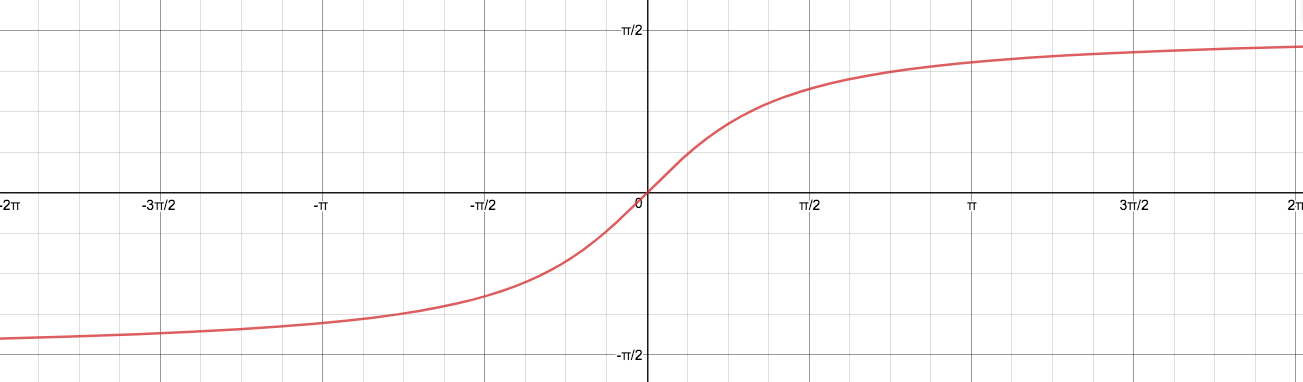
\includegraphics[width = 10 cm, height = 5 cm]{graph.png}
\end{center}
We can see that as $a$ and $b$ approaches $\infty$ they equal they equal $-\frac{\pi}{2}$ and $\frac{\pi}{2}$
and when we substitute these numbers back in to make $$\frac{\pi}{2}--\frac{\pi}{2}$$
which just equals $$\fbox{\pi}$$
 \\\underline{Example 3}
 $$\int\limits_{-3}^{1}\frac{x}{\sqrt{9-x^2}}dx$$
 In this problem we see that when $-3$ would be substituted in, the denominator would be $0$ so we have to take the limit to see what it would approach.
 $$\lim_{a\to-\-3}\int\limits_{a}^{1}\frac{xdx}{\sqrt{9-x^2}}dx$$
Then, we will integrate like any other problem. I'm going to bring the denominator up and then use u substitution.
$$\lim_{a\to-\-3}\int\limits_{a}^{1}{x{{(9-x^{2})}}^{\frac{-1}{2}}}dx$$
to integrate we will use u-substitution with $u$ being $9-x^2$ and $du$ being $2x$ 
$$\lim_{a\to-\-3}{\frac{1}{2}}\int\limits_{a}^{1}{{{(u)}}^{\frac{-1}{2}}}du$$
When we integrate this we get 
$$\frac{1}{2}{(9-x^{2})}^{\frac{1}{2}}|\limits_{a}^{1}$$
Now we can start substituting 
$$\lim_{a\to-\-3}{(9-1^2)}^{\frac{1}{2}}{-{(9-a^2)}^{\frac{1}{2}}}$$
As we think about how as $a$ increases from $0$ to $3$ we can make a chart 
\begin{tabular}{c|c}
     $x$ & $y=(9-x^2)^\frac{-1}{2}$ \\
    \hline
     $0 & 3 $ \\
     $1 & 2\sqrt{2} $\\ 
     $2 & \sqrt{5}$\\
     $2.5 & 1.6583$
     $2.75 & 1.19896$
     $2.99 & .2447$
 \end{tabular}
We can that it is approaching $0$ and $(8)^\frac{1}{2}$ is $2\sqrt{2}$ and $$2\sqrt{2}-0=\fbox{2\sqrt{2}}$$
\\ \underline{Example 4}
 $$\int\limits_{-2}^{0}\frac{4x}{(x+1)^2}dx$$ 
\begin{center}
    

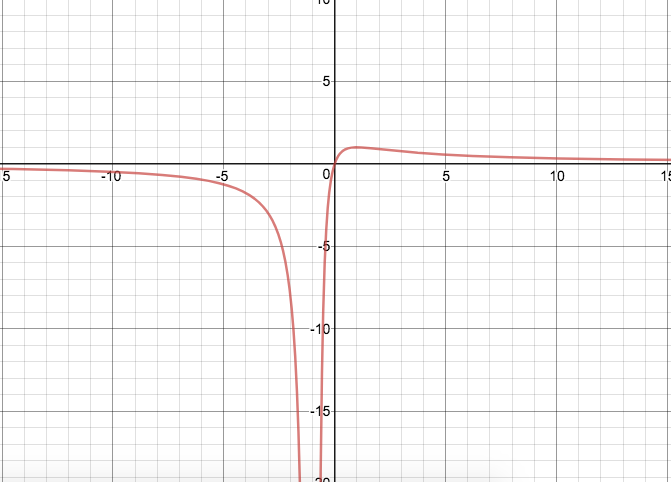
\includegraphics[width = 10 cm, height = 5 cm]{discontinuity.png}
\end{center}
 Because there is a point of discontinuity in this graph at $-1$ we have to break the original integrals into two at the point of discontinuity with the same equation like this 
 $$\int\limits_{-2}^{-1}\frac{4x}{(x+1)^2}dx + \int\limits_{-1}^{0}\frac{4x}{(x+1)^2}dx$$
We have to take the limit of negative one because if we didn't then it would make the denominator $0$ which would be undefined and makes it look like this
$$\limit_{b\to-\-1}\int\limits_{-2}^{b}\frac{4x}{(x+1)^2}dx + \limit_{a\to-\-1}\int\limits_{a}^{0}\frac{4x}{(x+1)^2}dx$$
Now we have to integrate both pieces which is really just one because it is the same equation.
With this equation we're going to use partial fractions making
$$\frac{a}{(x+1)}+\frac{b}{(x+1)^2}=\frac{4x}{(x+1)^2}$$
Then we have to find a common denominator which will be $(x+1)^2$, meaning that it will turn into this
$$\frac{a(x+1)}{(x+1)^2}+\frac{b}{(x+1)^2}=\frac{4x}{(x+1)^2}$$
To isolate a variable, we have to substitute a value in. In this case $x=-1$ it will be $b=-4$ and then when $x=0$ then $a+b=0$ and since $b=-4, a=4$ so 
$$\frac{4}{(x+1)}+\frac{-4}{(x+1)^2}=\frac{4x}{(x+1)^2}$$
and when we integrate this it equals $$(4\ln{(x+1)}+\frac{4}{x+1})|\limits_{-2}^{b}+(4\ln{(x+1)}+\frac{4}{x+1})|\limits_{a}^{0}$$
which is $$(4\ln{(b+1)}+\frac{4}{b+1}-(4\ln{(-2+1)}+\frac{4}{-2+1}))+(4\ln{(0+1)}+\frac{4}{0+1}-(4\ln{(a+1)}+\frac{4}{a+1}))$$
This simplified is
$$\lim_{\frac{a\to-\-1}{b\to-\-1}}(4\ln{(b+1)}+\frac{4}{b+1}+4\ln{(a+1)}\frac{4}{a+1})$$
since both limits are approaching $-1$ we are able to just say that $a=b$
 $$\lim_{a\to-\-1}(4\ln{(a+1)}+\frac{4}{a+1}+4\ln{(a+1)}-\frac{4}{a+1})$$
 when we simplify again it equals
 $$\lim_{a\to-\-1}(4\ln{(a+1)}+4\ln{(a+1)}$$
 which equals
 $-\infty+-\infty$ making \fbox{$-\infty$}
 \ssection{Differential Equations}
 \underline{Introduction}\\
 \\
 Differential equations are very true to their name; they're equations that contain a derivative. The problems can appear with the derivative in the form of $y'$ or $\frac{dy}{dx}$, depending on the type of the differential equation. To solve differential equations, the overall goal is to arrange the equation so that it can be integrated. We can graph differential equations using slope fields. We can also use differential equations and apply them to the real world by using the logistic model. 
 \section*{First Order Separable Differential Equations}
 For first order separable differential equations, we want the form of the derivative to be written as $\frac{dy}{dx}$. Separable differential equations are also very true to their name because of their ability to separate $x$ and $y$ to properly integrate the equation. All of the y's must be multiplied on the side of the derivative and the x's must be on the other side. To see this, let's start off with a basic example.\\
 Examples:\\
 \\
 \underline{Example 1}\\
 $$\frac{dy}{dx}=\frac{2x}{y}$$
 Since the end goal is to arrange the equation so that we can integrate it, we need to multiply both sides of the equation by y to make the left side easy to solve. 
 $$y\cdot \frac{dy}{dx}=\frac{2x}{y}\cdot y$$
 $$\int ydy =\int 2xdx$$
 Since we're also integrating with respect to x, separating the equation makes it easy to integrate the right side of the equation.
 $$\frac{1}{2}y^2+c=x^2+c$$
 Because we know that the c's on both sides are constants, we also know that we're able to combine them into one unknown constant on one side. 
 $$\frac{1}{2}y^2=x^2+c$$
 Now, try to isolate y by multiplying both sides by 2. Once again, c won't be affected because it's an unknown constant.
 $$2\cdot \frac{1}{2}y^2=(x^2+c)\cdot 2$$
 $$y^2=2x^2+c$$
 Take the square root of both sides to isolate y.
 $$\fbox{y=\pm \sqrt{2x^2+c}}$$
 Since this solution has the constant, c, in it, it's called a general solution. If we were given an initial condition along with the differential equation, we would've been able to solve for c. Let's try an example of this.\\
 \underline{Example 2}\\
 $$\frac{dy}{dx}=4xy\; \; \; y(0)=4$$
 $$\frac{1}{y}\cdot \frac{dy}{dx}=4xy\cdot \frac{1}{y}$$
 Separate by multiplying by the y's as usual.
 $$\int \frac{1}{y}dy=\int 4xdx$$
 Integrate.
 $$ln|y|+c=2x^2+c$$
 Combine the c values.
 $$ln|y|=2x^2+c$$
 In order to isolate y, we have to put each side of the equation as a power of $e$ so that $e^{ln|y|}$ will just become y.
 $$e^{ln|y|}=e^{2x^2+c}$$
 $$y=e^{2x^2+c}$$
 We can rewrite $e^{2x^2+c}$ because of the understanding that when two bases of the same number or constant are multiplied, their exponents are added.
 $$y=e^{2x^2}\cdot e^c$$
 Since we know that $e$ to some power is going to be a constant, we can rewrite $e^c$ as c.
 $$\fbox{y=c\cdot e^{2x^2}}$$
 This is the general solution. Since we have an initial condition as a part of the problem, or a value for y when x is 0, we can solve to find a value for c. All we have to do is substitute 0 for x and 4 for y.
 $$4=c\cdot e^{2\cdot(0)^2}$$
 $$4=c\cdot e^{2\cdot 0}$$
 $$4=c\cdot e^{0}$$
 $$4=c\cdot 1$$
 $$4=c$$
 Now we can substitute our newly found c value into the equation.
 $$\fbox{y=4\cdot e^{2x^2}}$$
 This equation with a number instead of c is called a particular solution. This is what you want to solve for when you're given an initial condition. \\
 \underline{Example 3}\\
 $$\frac{dy}{dx}=e^{x+ln(y^2)}\; \; \; y(0)=\frac{1}{2}$$
 We can use the same idea about bases of the same number and when their exponents are added to rewrite this equation.
 $$\frac{dy}{dx}=e^x\cdot e^{ln(y^2)}$$
 Simplify.
 $$\frac{dy}{dx}=e^x\cdot y^2$$
 $$\frac{1}{y^2}\cdot \frac{dy}{dx}=e^x\cdot y^2 \cdot \frac{1}{y^2}$$
 Integrate.
 $$\int \frac{1}{y^2}dy=\int e^xdx$$
 $$-\frac{1}{y}+c=e^x+c$$
 Combine c values.
 $$-\frac{1}{y}=e^x+c$$
 Divide by negative one to isolate y. We still write c with an addition sign because it's still an unknown constant. 
 $$\frac{1}{y}=-e^x+c$$
 Multiply each side of the equation to the $-1$ power to flip the fraction on the left side and fully isolate y.
 $${\frac{1}{y}}^{-1}=(-e^x+c)^{-1}$$
 $${y=\frac{1}{e^x+c}}$$
 This is the general solution. Now we have to solve for the particular solution.
 $$\frac{1}{2}=\frac{1}{e^0+c}$$
 $$\frac{1}{2}=\frac{1}{1+c}$$
 $$c=1$$
 $$y=\frac{1}{e^x+1}$$
This is the particular solution.
$$\fbox{y=(e^x+1)^{-1}}$$
This is another way of writing the particular solution (so that it could fit in a text box).\\
\\
\underline{Example 4}
$$\frac{dy}{dx}=xy+2x$$
At first it seems like we can't move the y's to the left side, but we actually can. Let's try factoring an $x$ out of the right side.
$$\frac{dy}{dx}=x(y+2)$$
Now we can divide both sides by $y+2$.
$$\frac{1}{y+2}\frac{dy}{dx}=x$$
Integrate.
$$\int \frac{1}{y+2}dy=\int xdx$$
For the integration on the left, we'll have to use u-substitution. 
$$(u=y+2\longrightarrow du=dy)$$
$$\int \frac{1}{u}du=\frac{1}{2}x^2+c$$
Integrate.
$$ln|u|+c=\frac{1}{2}x^2+c$$
Substitute the u-value in and combine the c values.
$$ln|y+2|=\frac{1}{2}x^2+c$$
Put each side to the power of $e$.
$$e^{ln|y+2|}=e^{\frac{1}{2}x^2+c}$$
Simplify.
$$y+2=e^{\frac{1}{2}x^2+c}$$
We can rewrite $e^{\frac{1}{2}x^2+c}$ because of the understanding that when two bases of the same number or constant are multiplied, their exponents are added.
$$y+2=e^{\frac{1}{2}x^2}\cdot e^c$$
Rewrite $e^c$ as a constant.
$$y+2=ce^{\frac{1}{2}x^2}$$
Isolate $y$.
$$\fbox{y=ce^{\frac{1}{2}x^2}-2}$$
 \section*{First Order Linear Differential Equations}
 For first order linear differential equations, we want the form of the derivative to be $y'$. These differential equations have the derivative plus the y's on the left side of the equation and other information on the right. We'll use a process, called the integrating factor, which capitalizes on our knowledge of the product rule. Since we know that $f'\cdot g+f\cdot g'=(f\cdot g)'$, we will try to arrange our differential equation to this setup so that we can easily integrate it. Let's see this more clearly in some examples.\\
  Examples:\\
 \\
 \underline{Example 1}\\
 $$y'+2xy=x$$
 Since our equation is already in ideal form, we can go ahead and multiply it by a variable, m. We do this to discover what value of m satisfies $f'\cdot g+f\cdot g'=(f\cdot g)'$.
 $$my'+2xmy=mx$$
 Because we know that we want the information being multiplied by y (2m) to be equal to m', we will set them equal to each other.
 $$2xm=m'$$
 Isolate the m's to one side so that we can easily integrate both sides of the equation.
 $$2x=\frac{m'}{m}$$
 $$\int 2xdx=\int \frac{m'}{m}dx$$
 To integrate m, we'll have to use u-substitution.
 $$(u=m\longrightarrow du=m'dx)$$
 $$x^2+c=\int \frac{1}{u}du$$
 $$x^2+c=ln|u|+c$$
 $$x^2+c=ln|m|+c$$
 Now we're not exactly sure what c is, but we know that it can equal any value. So, to make the process simpler, let's set c equal to 0.
 $$x^2=ln|m|$$
 To isolate m, put each side to the power of $e$.
 $$e^{x^2}=e^{ln|m|}$$
 $$e^{x^2}=m$$
 Now we can substitute this value back into our original equation with m in it.
 $$e^{x^2}y'+2xe^{x^2}y=e^{x^2}x$$
 Since we have our equation rewritten in the product rule form that we were searching for, we can rearrange our equation.
 $$\int (e^{x^2}\cdot y)'dx=\int e^{x^2}xdx$$
 The left side is easy to integrate, but the right side is going to require u-substitution.
 $$x^2=u\longrightarrow 2xdx=du\longrightarrow xdx=\frac{1}{2}du$$
 $$e^{x^2}\cdot y+c=\frac{1}{2}\int e^udu$$
 $$e^{x^2}\cdot y+c=\frac{1}{2}e^u+c$$
 $$e^{x^2}\cdot y+c=\frac{1}{2}e^{x^2}+c$$
 Combine c values.
 $$e^{x^2}\cdot y=\frac{1}{2}e^{x^2}+c$$
 Isolate y to get the general solution.
 $$y=\frac{1}{2}(\frac{e^{x^2}}{e^{x^2}})+\frac{c}{e^{x^2}}$$
 $$\fbox{y=0.5+ce^{-x^2}}$$
 \underline{Example 2}\\
 $$y'=3+y\; \; \; y(0)=2$$
 For this problem, we have to rearrange the equation to get y on the left side.
 $$y'-y=3$$
 Now, we have to be careful that we follow the product rule when solving this problem, so we should change our signs a bit to make solving easier.
 $$y'+(-y)=3$$
 Multiply by m.
 $$my'+(-my)=3m$$
 $$-m=m'$$
 $$-1=\frac{m'}{m}$$
 Integrate.
 $$\int -1dx=\int \frac{m'}{m}dx$$
 $$-x+c=ln|m|+c$$
 Once again, allow c to equal 0.
 $$-x=ln|m|$$
 Put both sides to the power of $e$.
 $$e^{-x}=e^{ln|m|}$$
 $$e^{-x}=m$$
 Substitute m into the original equation.
 $$e^{-x}y'+(-e^{-x}y)=3e^{-x}$$
 Rearrange the equation based on our knowledge of the product rule.
 $$(e^{-x}\cdot y)'=3e^{-x}$$
 Integrate.
 $$\int (e^{-x}\cdot y)'dx=\int 3e^{-x}dx$$
 $$e^{-x}\cdot y+c=-3e^{-x}+c$$
 Combine c values.
 $$e^{-x}\cdot y=-3e^{-x}+c$$
 Isolate y.
 $$y=-3(\frac{e^{-x}}{e^{-x}})+\frac{c}{e^{-x}}$$
 $$\fbox{y=-3+ce^{x}}$$
 This is the general solution. Since we have an initial condition, we need to find a particular solution.
 $$2=-3+ce^0$$
 $$5=c$$
 Now, substitute this into the general solution to find the particular solution.
 $$\fbox{y=-3+5e^{x}}$$
 \underline{Example 3}\\
 $$x^2y'+xy=1$$
 In order to solve linear differential equations, there must be no value other than 1 in front of y'. Since there is in this problem, we must get y' by itself by dividing by $x^2$.
 $$y'+\frac{x}{x^2}y=\frac{1}{x^2}$$
 $$y'+\frac{1}{x}y=\frac{1}{x^2}$$
 Now multiply by m.
 $$my'+\frac{m}{x}y=\frac{m}{x^2}$$
 $$\frac{m}{x}=m'$$
 $$\frac{1}{x}=\frac{m'}{m}$$
 Integrate.
 $$\int \frac{1}{x}dx=\int \frac{m'}{m}dx$$
 $$ln|x|+c=ln|m|+c$$
 Let c equal 0.
 $$ln|x|=ln|m|$$
 Put both sides to the power of $e$.
 $$e^{ln|x|}=e^{ln|m|}$$
 $$x=m$$
 Substitute back into the original equation.
 $$xy'+\frac{x}{x}y=\frac{x}{x^2}$$
 $$xy'+y=\frac{1}{x}$$
 Using our knowledge of the product rule, let's rewrite this.
 $$(x\cdot y)'=\frac{1}{x}$$
 $$\int (x\cdot y)'dx=\int \frac{1}{x}dx$$
 $$x\cdot y=ln|x|+c$$
 Isolate y.
 $$y=\frac{ln|x|}{x}+\frac{c}{x}$$
 $$\fbox{y=ln|x|\cdot x^{-1}+c\cdot x^{-1}}$$
 \section*{Slope Fields}
  Intro: Using implicit differential equations such as $\frac{dy}{dx}=x+y$ we can plot lines at each point on a graph. These scatter plots of different slopes are called slope fields which are used to find the general solution to implicit differential equations.\\
 \\
 \underline{Example 1}\\
 $$\frac{dy}{dx}=x+y$$ 
This differential equation gives us a slope at any specific point on the xy plane. So let's take a look at a specific point (1,1). In order to find the slope of the tangent line all you have to do is substitute in the the y values for the respective y values and the x values for the respective x values like this...\\
$$\frac{dy}{dx}=x+y,\frac{dy}{dx}=1+1,\frac{dy}{dx}=2$$\\
Now that we have this set up down let's graph a whole bunch of tangent lines from the domain and range of $-2\leq x\leq2, -2\leq y\leq 2$. Don't forget to show your work on how you got there. Note: an easy way to is to create a table of values.\\\\

 
    Table for $\frac{dy}{dx}=x+y$\\
 \begin{tabular}{c|c|c|c|c|c|c}
     &&&&\fbox{x}&&\\
    \hline
     &&\fbox{-2}&\fbox{-1}&\fbox{0} &\fbox{1}&\fbox{2}\\
    \hline
     &\fbox{-2}&-4&-3&-2&-1&0\\
    \hline
    \fbox{y}&\fbox{-1}&-3&-2&-1&0&1\\
    \hline
     & \fbox{0}&-2&-1&0&1&2\\
    \hline
     & \fbox{1}&-1&0&1&2&3\\
    \hline
      & \fbox{2}&0&1&2&3&4\\
 \end{tabular}
 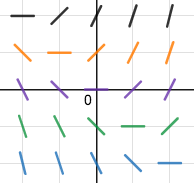
\includegraphics[width = 4 cm, height = 4 cm]{SF1.png}

 \\
 Let's do some more examples just to show how easy it is to apply slope fields to graphs\\\\\\\\
 \underline{Example 2}\\
 \\
 $$\frac{dy}{dx}=\frac{2x}{y}, -2\leq x\leq2, -2\leq y\leq 2$$ \\
 \begin{tabular}{c|c|c|c|c|c|c}
     &&&&\fbox{x}&&\\
    \hline
     &&\fbox{-2}&\fbox{-1}&\fbox{0} &\fbox{1}&\fbox{2}\\
    \hline
     &\fbox{-2}&2&1&0&-1&-2\\
    \hline
    \fbox{y}&\fbox{-1}&4&2&0&-2&-4\\
    \hline
     & \fbox{0}&Und&Und&Und&Und&Und\\
    \hline
     & \fbox{1}&-4&-2&0&2&4\\
    \hline
      & \fbox{2}&-2&-1&0&1&2\\
 \end{tabular}
 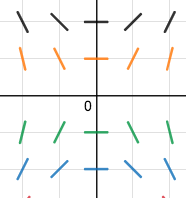
\includegraphics[width = 4 cm, height = 4 cm]{SF2.png}\\\\
 \underline{Example 3}\\
   $$\frac{dy}{dx}=x^y, -2\leq x\leq2, -2\leq y\leq 2$$ \\
    \begin{tabular}{c|c|c|c|c|c|c}
     &&&&\fbox{x}&&\\
    \hline
     &&\fbox{-2}&\fbox{-1}&\fbox{0} &\fbox{1}&\fbox{2}\\
    \hline
     &\fbox{-2}&$\frac{1}{4}$&$1$&DNE&1&$\frac{1}{4}$\\
    \hline
    \fbox{y}&\fbox{-1}&$\frac{1}{-2}$&1&DNE&1&$\frac{1}2{}$\\
    \hline
     & \fbox{0}&1&1&1&1&1\\
    \hline
     & \fbox{1}&2&1&0&1&2\\
    \hline
      & \fbox{2}&4&1&0&1&4\\
 \end{tabular}
 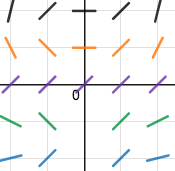
\includegraphics[width = 4 cm, height = 4 cm]{SF3.png}\\
 \\\\
 Conclusion-\\
 Although very basic and very easy to create, slope fields are very useful. They plot out a general solution or all solutions for the differential equation and let us estimate what the line or function is without doing any work to solve for anything.
 \section*{Euler's Method}
  Intro: When given implicit differentiated equations that are hard to integrate into their original forms we can use the idea of finding a slope fields to helps us. For example
  
  Using implicitly differentiated equations with given initial values we can estimate any other value for that specific solution without having to use integration. In Euler's method we use lots of steps to get approximate values for certain points. The more steps there is, the closer we can get to the actual value.\\
  
 \\
 \underline{Example 1}\\
 \\
 $\frac{dy}{dx}=2x-y,y(0)=3,$ with steps of h=.5 on the interval from $0\leq x\leq 1$\\
 In order to start the question above we need to begin with the initial value given to us $y(0)=3$. Substitute it into the differential equation to find our first slope.
 $$\frac{dy}{dx}=2(0)-3=3$$\\
 Now that we have the slope lets create an equation for the tangent line at that point.
 $$y-3=-3x$$
 Substitute in our next x value which is .5 in order to complete our next point in the problem.
 $$y(.5)=-3\cdot.5+3$$
 $$y(.5)=1.5$$
 Now that we have a new point of (.5,1.5) we can substitute this into our differential equation.
 $$\frac{dy}{dx}=2(.5)-1.5,\frac{dy}{dx}=-.5$$
 Let's create another tangent line with our given slope. Then substitute in one to find our final y value.\\
 $$y-1.5=-0.5(x-0.5)$$
  $$y(1)=-0.5(0.5)+1.5$$
  $$\fbox{y(1)=1.25}$$
 Our final answer for the Euler's method is 1.25.
 Let's find the percent error and see the comparison to the actual value. Use integration now.\\
 $$\frac{dy}{dx}=2x-y$$
 $$\frac{dy}{dx}+y=2x$$
 Let's use an integrating factor in order to solve for this one.
 $$(\frac{dy}{dx}+y=2x)m$$
 $$m\cdot\frac{dy}{dx}+m\cdot y=m\cdot2x$$
 Solve for m using the fact that $m'$ equals $m$
 $$m'=m$$
 $$\frac{m'}{m}=1$$
  $$\int\frac{m'}{m}dm=\int(1)dx$$
  $$\ln{m}=x$$
  $$m=e^x$$
  Substitute that back in to the equation and integrate.
   $$e^x \cdot\frac{dy}{dx}+e^x \cdot y=e^x \cdot2x$$
   $$(e^x \cdot y)'=e^x \cdot2x$$
   $$\int(e^x \cdot y)'dx=\int e^x \cdot2x dx$$
   
   $$e^x \cdot y=2xe^x-2e^x+c$$
    $$y=2x-2+ce^{-x}$$
Substitute the initial condition in (0,3) to solve for c
$$3=2(0)-2+ce^0$$
$$3+2=c=5$$
Now use the c value to back into the equation and then substitute in 1 for x.
$$y=2(1)-2+5e^{-1}$$
$$\fbox {y\approx1.8394}$$
Now let's calculate percent error.
$$\frac{|1.8394-1.25|}{1.8394} \cdot 100\%\fbox{\approx32.043\%}$$
The percent error seems to be quite high when we use two steps. Let's try 10 steps with a step value of point one. We should probably use a table for this one.\\\\
\begin{tabular}{c|c|c}
     Point&Slope &Equation \\
\hline
    (0,3 )&$\frac{dy}{dx}=2(0)-3=-3$ &$y_1-3=-3(x-0)$ \\
    (0.1, $y_1(0.1)=2.7$) &$\frac{dy}{dx}=2(0.1)-2.7=-2.5$ &$y_2-2.7=-2.5(x-0.1)$ \\
    (0.2, $y_2(0.2)=2.45$) &$\frac{dy}{dx}=2(.2)-2.45=-2.05$ &$y_3-2.45=-2.05(x-0.2)$ \\
    (0.3, $y_3(0.3)=1.845$) &$\frac{dy}{dx}=2(.3)-1.845=-1.245$ &$y_4-1.845=-1.245(x-0.3)$ \\
    (0.4, $y_4(0.4)\approx1.721$) &$\frac{dy}{dx}=2(.4)-1.721\approx-0.921$ &$y_5-1.721=-0.921(x-0.4)$ \\
    (0.5, $y_5(0.5)\approx1.628$)&$\frac{dy}{dx}=2(.5)-1.628\approx-0.628$ &$y_6-1.628=-0.628(x-0.5)$ \\
    (0.6 ,$y_6(0.6)\approx1.565$) &$\frac{dy}{dx}=2(.6)-1.565\approx-0.365$ &$y_7-1.565=-0.365(x-0.6)$ \\
    (0.7, $y_7(0.7)\approx1.528$) &$\frac{dy}{dx}=2(.7)-1.528\approx-0.129$ &$y_8-1.528=-0.129(x-0.7)$ \\
    (0.8, $y_8(0.8)\approx1.516$) &$\frac{dy}{dx}=2(.8)-1.516\approx.084$ &$y_9-1.516=0.084(x-0.8)$ \\
    (0.9, $y_9(0.9)\approx1.524$) &$\frac{dy}{dx}=2(.9)-1.524\approx0.276$ &$y_{10}-1.524=0.276(x-0.9)$ \\
    (1, $y_{10}(1)\approx1.552$ )& & \\
    
\end{tabular}\\\\
Percent Error 
$$\frac{|1.8394-1.552|}{1.8394} \cdot 100\%\approx15.635\%$$
As you can see the percent error starts to decrease when we have more steps into the interval.
\\ \underline{Example 2}\\
 \\
 Let's look at another problem on the interval $0\leq x\leq 1$ with steps of 0.25.
 $$\frac{dy}{dx}=x+y,\; y(0)=1$$
 To start this equation, we have to begin with the initial value. Substitute it into the original equation to find the slope.
 $$\frac{dy}{dx}=0+1=1$$
 Now that we have the slope, let's create a tangent line for the point.
 $$y-1=1(x)$$
 Now, let's substitute our next step value in.
 $$y-1=1(0.25)=1.25$$
 We find that the new y value is 1.25. Let's substitute our new x and y values into the differential equation to find the slope.
 $$\frac{dy}{dx}=.25+1.25=1.5$$
 Let's use this slope to create a new equation.
 $$y-1.25=1.5(x-0.25)$$
 Substitute the next x value in to find the new y value.
 $$y-1.25=1.5(0.5-0.25)=1.625$$
 Let's use the new x and y values to find the slope at this point.
 $$\frac{dy}{dx}=0.5+1.625=2.125$$
 Now that we have the slope, let's create another tangent line.
 $$y-1.625=2.125(x-0.5)$$
 Let's substitute our next x value in.
 $$y-1.625=2.125(0.75-0.5)=2.15625$$
 Let's use these values to find the new slope.
 $$\frac{dy}{dx}=0.75+2.15625=2.90625$$
 We can use this information to create our last tangent line.
 $$y-2.15625=2.90625(x-0.75)$$
 Now we can substitute our last x value in to find the estimated value for 1 in the equation.
 $$y-2.15625=2.90625(1-0.75)=2.8828125$$
 $$\fbox{y(1)=2.8828125}$$.
 \underline{Table of our steps}\\
 \begin{tabular}{c|c|c}
     Point&Slope &Equation \\
\hline
    (0,1)&$\frac{dy}{dx}=0+1=1$ &$y_1-1=1(x-0)$ \\
    (0.25, $y_1(0.25)=1.25$) &$\frac{dy}{dx}=0.25+1.25=1.5$ &$y_2-1.25=1.5(x-0.25)$ \\
    (0.5, $y_2(0.5)=1.625$) &$\frac{dy}{dx}=1.625+0.5=2.125$ &$y_3-1.625=2.125(x-0.5)$ \\
    (0.75, $y_3(0.75)=2.15625$) &$\frac{dy}{dx}=0.75+2.15625=2.90625$ &$y_4-2.15625=2.90625(x-0.75)$ \\
    (1, $y_4(1)=2.8828125$) &&
    
\end{tabular}\\\\\\\
Given that the integral to the differential equation with the Initial condition is $y=2e^x-x-1$ solve for the percent error from our estimated value of x=1 and actual value.
$$y(1)=2e^1-1-1\approx\fbox{3.43656}$$
$$\frac{3.43656-2.8828125}{3.43656}\cdot 100\%\fbox{\approx16.1135\%}$$
 \\\\
 \section*{Logistic Model}
 The logistic model was created to use differential equations that correspond to how the real world works. It makes a population able to die instead of constantly growing with no consequence by having capacity that it can achieve but not go over. Unlike an exponential graph, a logistic model graph will level off.
 The rate of change of a population is directly proportional to the amount present and to the difference of a constant and the amount present.
 proof: the original equation it comes from is $$\frac{dy}{dx}(m-y)$$ is where $k$ is the growth factor, $m$ is the carrying capacity, $$\frac{dy}{dx}$$ is the rate of change of a population, and $y$ is amount present.
 To find what $y$ equals we have to find the integral of the original equation so we will separate it like this 
 $$\int\frac{1}{y(m-y)}dy=\int(k)dt$$
 and now we can use partial fractions to separate the equation so we can integrate like this 
 $$\frac{1}{y(m-y)}=\frac{a}{y}+\frac{b}{m-y}$$
 and then when we create a common denominator it makes this
 $$\frac{1}{y(m-y)}=\frac{a(m-y)}{y(m-y)}+\frac{by}{y(m-y)}$$
 and when we substitute $0$ in for $y$ then we see that $1=am$ so that means $a=\frac{1}{m}$ and when we substitute a back in it equals this
 $1-\frac{y}{m}+by=1$ and that simplified is $\frac{y}{m}=by$ and when we divide $y$ from both sides $b$ also equals $\frac{1}{m}$ and when we put $a$ and $b$ back into the original equation we get this
 $$\int(\frac{\frac{1}{m}}{y}+\frac{\frac{1}{m}}{m-y})=\int kdt $$
 and we can take out $\frac{1}{m}$ so it makes
  $$\frac{1}{m}\int(\frac{1}{y}+\frac{1}{m-y})=\int kdt $$
  and the integral of that is $$\frac{1}{m}(lny-ln(m-y)=kt+c$$
  and we can simplify that into
  $$ln\frac{y}{(m-y)}=mkt+c$$
  To get rid of the natural log we can put both sides as the exponent of $e$ making
  $$e^{ln\frac{y}{(m-y)}}=e^{mkt+c}$$
  and since c is just a constant we were able to bring it down making
  $$ln\frac{y}{(m-y)}=ce^{mkt}$$
  Now we will substitute $\frac{y}{m-y}=v$ and $v=ce^{mkt}$and then isolate $y$ so $y=vm-vy$ so $y+vy=vm$ and we can take a $y$ out to be $y(1+v)+vm$ so $y=\frac{vm}{1+v}$ multiplied by $\frac{1}{v}$ making $\frac{m}{\frac{1}{v}+1}=y$
  and when we substitute them back it we make our  general logarithmic equation $$y(t)=\frac{m}{1+ce^{-mkt}}$$
  and to find c we say $y(0)=y_0$
  and $y_0=\frac{m}{1+c}$ and $m=y_0+y_0c$ and $y_0c=m-y_0$ and $c=\frac{m}{y_0}-1$ and when we substitute that into the general solution, we get the particular solution of 
  $$y(t)=\frac{m}{1+\frac{m}{(y_0}-1)e^{-mkt}}$$
  and to make it easier to use we multiply the whole equation by $y_0$ making
    $$y(t)=\frac{{my_0}}{{y_0+(m-y_0})e^{-mkt}}$$
    The other equation for a logistic model starts with the equation
$$\frac{dy}{dx}=ky(1-\frac{y}{l})$$ and that when integrated is this 
$$y(t)=\frac{{my_0}}{{y_0+(m-y_0})e^{-kt}}$$ this just eliminates the constant.
 \\Now we can start using these equations to solve some real life problems.\\
 \\
  \underline{Example 1}\\
 \\If there was a group of 56 dinosaurs living together, but their ecosystem could only support 70 and after 2 years there were 63 dinosaurs, how many dinosaurs will there be in three years, and when will they reach it‘s carrying capacity?
 \\First we can substitute our given information into the equation so $$63=\frac{70*56}{56+(70-56)e^{-2k}}$$ and when we calculate what we get for the growth factor we get $k=-ln(1.5)-.4055$ we can now use this number to calculate the amount of dinosaurs in three years by substituting our new information in to make $$y(3)=\frac{70*56}{56+(70-56)e^{3(-ln(1.5)}}$$ 
  \begin{center}
    

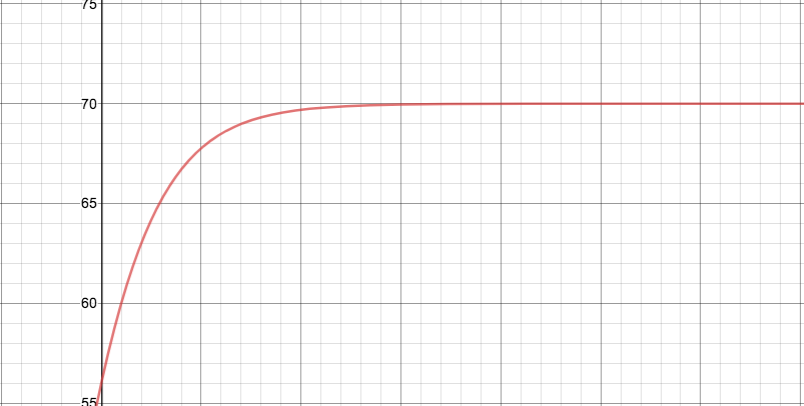
\includegraphics[width = 10 cm, height = 5 cm]{chicken.png}
\end{center}
 this comes out as being $y=65.1724=65$ dinosaurs. Because the graph of a logistic model forms an asymptote approaching the carrying capacity it will never actually reach $70$ dinosaurs so the when it closest reaches $70$ will give a good approximation like if we use $69.9$. It will take $12.7344$ years until the population reaches its carrying capacity.
 \\
 \underline{Example 2}\\ with this one we will analyze a logistic model graph and see what we can tell from it and then we will solve when the population reaches half of the carrying capacity if $k=.9$
 Here is a graph with the $x-axis$ being time (days) and the $y-axis$ being population
  \begin{center}
    

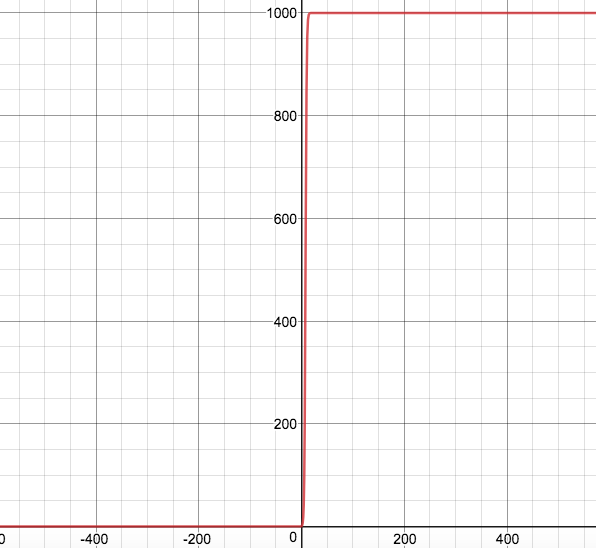
\includegraphics[width = 10 cm, height = 5 cm]{house.png}
\end{center}
 \\We see that the graph levels out at a point, this is the carrying capacity and which looks like it's at about $1000$ we see initially there is a population of of 1 because it hits the graph $x=0$ at $(y=1)$ and since we know this we can start building the equation of $$y(t)=\frac{(1)(1000)}{1+(1000-1)e^{-kt}}$$
 and now we can solve what the problem is looking for because we know $k$ and because half of the carrying capacity is just $500$ so
 
 $$500=\frac{1000}{1+999e^{-.9t}}$$
 we then get rid of the denominator by multiplying by the denominator and then dividing by $500$ to make
 $$1+999e^{-.9t})=2$$ we then subtract $1$ and divide by $999$ to make
 $e^{-.9t}=\frac{1}{999}$
 and then we take the natural log to get rid of the exponent making $$-.9t=ln(frac{1}{999})$$
 and then that meant $t=7.67417$
 
 \underline{Example 3}\\ There are 37 flies put into a container and after being left out there are 87, if the growth rate is .7863 then how long was the group of flies left out for and if there can only be 248 flies in the area at a time how long until half of their limit is reached?
 \\when we substitute these numbers into the equation we get $$\frac{(37)(248)}{37+(248-37)e^{-.7863t}}=87$$ 
 when this is solved it takes 1.4313 days for the flies to reach this number and to find when half their carrying capacity you just have to the equation equal to half of $248$ so $124$ like this  
 $$\frac{(37)(248)}{37+(248-37)e^{-.7863t}}=124$$ which is 2.2141 days. 
\end{document}
